\section{Tests}
We performed some basic tests for the DNS service and the new policy that were enabled and implemented in this assignment.\\
To perform thorough tests on the firewall rules we implemented, the WAN interface on the \textbf{Main router} was enabled, through the option provided in OPNSense, to accept private connections, so that it could be reached from external hosts (Internet, or our local machines).\\

\subsection{Testing the DNS Service}
For the internal DNS service, once defined all the firewall rules, we just tried to solve the domain names through the \textbf{host} command on terminal on the machines exploiting the service, verifying that the names were correctly solved to their corresponding IP addresses - e.g., \textit{coffee.acme.group27}, \textit{dc.acme.group27} or \textit{web.acme.group27} were correctly resolved by any machine in \textbf{DMZ subnet} and \textbf{Clients network} subnet. The same command was then run on machinesd of the \textbf{external clients subnet}, verifying that some external domain names were correctly resolved - e.g., \textit{google.com}.\\
No errors or misconfiguration problems were faced during this test phase.

\subsection{Testing the policy}
To test the policy implementation and make sure it behaves the way we wanted it to behave as described in the third paragraph, we had to perform some basic tests by exploiting at least one machine in each of our subnetworks, and also an external one on the \textbf{WAN interface} simulating an external machine connected from the Internet.\\
A bunch of basic tests consisted in \textit{pinging} internal or external machines (not in the same LANs obviously), since ICMP is not mentioned in the policy and thus it should be disabled by default - indeed, the ouctomes were always negative: no machine in the target network is able to ping any other machine that is not in the same LAN.\\
The pictures showed below represent, for each point of the policy that was implemented, a testing command that was executed - either via terminal or via browser - and its corresponding desired output.\\

\begin{figure}[H]
\centering
\begin{minipage}{.5\textwidth}
  \centering
  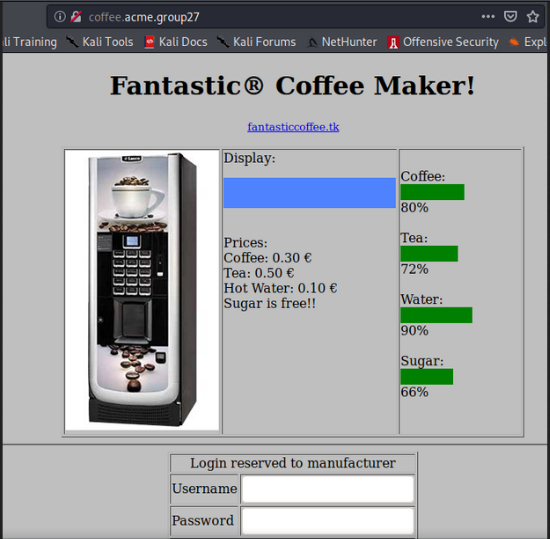
\includegraphics[width=1\textwidth]{clientCanConnectToHTTPExt.png}
  \caption[a]{Machine in Clients subnet can connect via HTTP/HTTPS to web service in External Clients subnet.}\label{fig:1}
\end{minipage}%
\begin{minipage}{.5\textwidth}
  \centering
  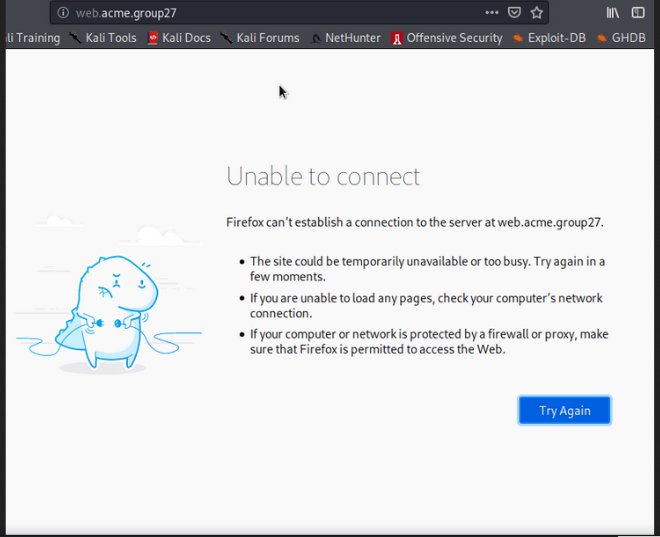
\includegraphics[width=1\textwidth]{clientOtherHTTPDisabled.png}
  \caption[a]{Machine in Clients subnet cannot connect via HTTP/HTTPS to any other web service that is not in External Clients subnet, not even in DMZ.}\label{fig:2}
\end{minipage}
\end{figure}

\begin{figure}[H]
\centering
\begin{minipage}{.5\textwidth}
  \centering
  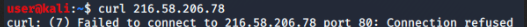
\includegraphics[width=1\textwidth]{clientCANNOTGoOut.png}
  \caption[a]{Machine in Clients subnet cannot connect via HTTP/HTTPS outside (WAN).}\label{fig:3}
\end{minipage}%
\begin{minipage}{.5\textwidth}
  \centering
  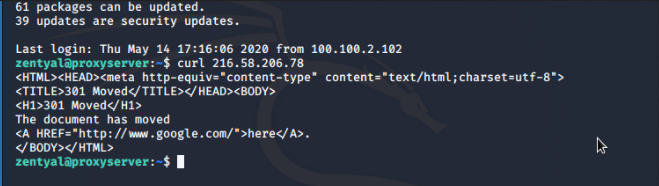
\includegraphics[width=1\textwidth]{proxyCanGoOutToHaveFun.png}
  \caption[a]{Proxy machine is enabled to connect via HTTP/HTTPS to Google, outside (WAN).}\label{fig:4}
\end{minipage}
\end{figure}

\begin{figure}[H]
\centering
\begin{minipage}{.5\textwidth}
  \centering
  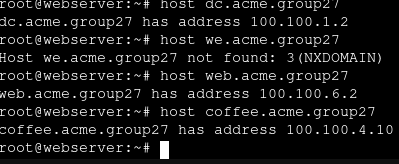
\includegraphics[width=1\textwidth]{dnsWorkingWebServer.png}
  \caption[a]{Web server (DMZ) can DNS request on Domain Controller machine.}\label{fig:5}
\end{minipage}%
\begin{minipage}{.5\textwidth}
  \centering
  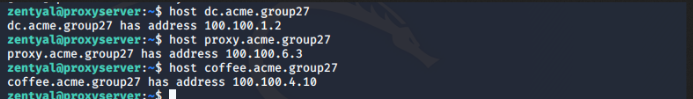
\includegraphics[width=1\textwidth]{DMZCanuseDNSService.png}
  \caption[a]{Same for Proxy (DMZ).}\label{fig:6}
\end{minipage}
\end{figure}

\begin{figure}[H]
\centering
\begin{minipage}{.5\textwidth}
  \centering
  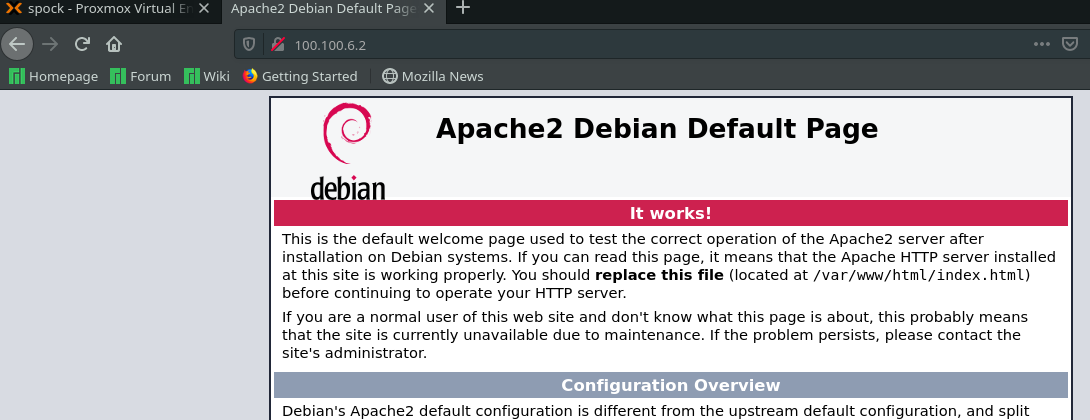
\includegraphics[width=1\textwidth]{web_reachableHTTP.png}
  \caption[a]{Web server (DMZ) is reachable from the outside (WAN) on HTTP/HTTPS protocol.}\label{fig:7}
\end{minipage}%
\begin{minipage}{.5\textwidth}
  \centering
  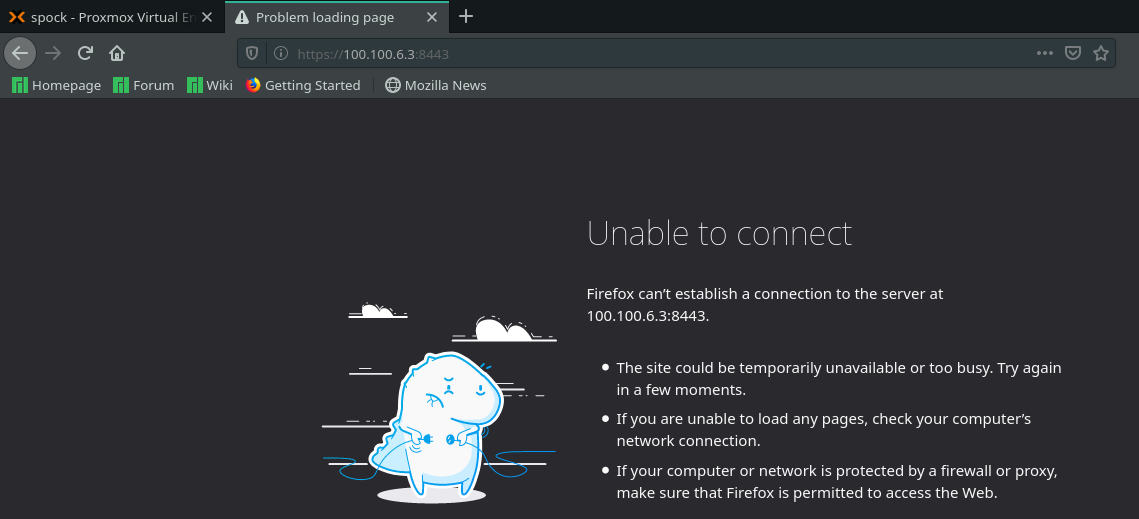
\includegraphics[width=1\textwidth]{firewallShieldingProxyZentyal.png}
  \caption[a]{Proxy is not reachable from outside, not even on its Zentyal service port.}\label{fig:8}
\end{minipage}
\end{figure}

\begin{figure}[H]
\centering
  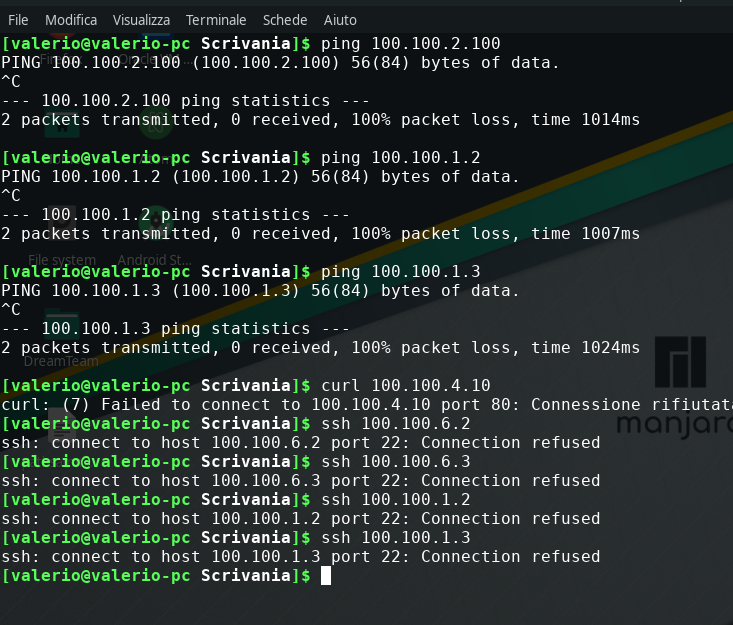
\includegraphics[width=1\textwidth]{WANRefusingUndesiredConnections.png}
  \caption[a]{WAN interface rejecting connections to specific hosts in the target network on specific protocols.}\label{fig:9}
\end{figure}

Please notice also that in some of these tests we were able to perform an SSH connection and authentication on some of the machines in the DMZ from the \textbf{Kali machine}: we indeed verified that machines in DMZ and Internal Services network accept connections on port 22 from the Clients network only, while they reject any other connection on the very same port from different source networks.
